\subsection{UCW4 - Area Personale}
\begin{figure}[!h]
\centering
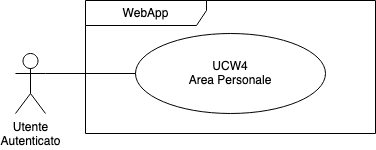
\includegraphics[scale=0.5]{UC_images/UCW4.png}
\caption{UCW4 - Area Personale}
\end{figure}
\begin{itemize}
\item \textbf{Descrizione}: L'utente è autenticato nella piattaforma Sweeat e accede alla sua Area Personale.
\item \textbf{Attore primario}: Utente Autenticato.
\item \textbf{Precondizione}: L'utente è autenticato nella piattaforma.
\item \textbf{Postcondizione}: L'utente accede alla sua area personale per gestire il suo profilo.

\item \textbf{Scenario principale}:
\begin{enumerate}
\item L'utente autenticato clicca l'icona per accedere alla sua Area Personale;
\item Una volta entrato nell'Area Personale, può gestire il suo profilo.
\end{enumerate}

\item \textbf{Sottocasi}:
\begin{enumerate}
	\item Collegare l'account personale di Instagram (UCW4.1 \S 3.5.1).
	\item Collegare l'account personale di TikTok (UCW4.2 \S 3.5.2).
	\item Modificare la password (UCW4.3 \S 3.5.3). 
\end{enumerate}
\end{itemize}
\begin{figure}[!h]
\centering
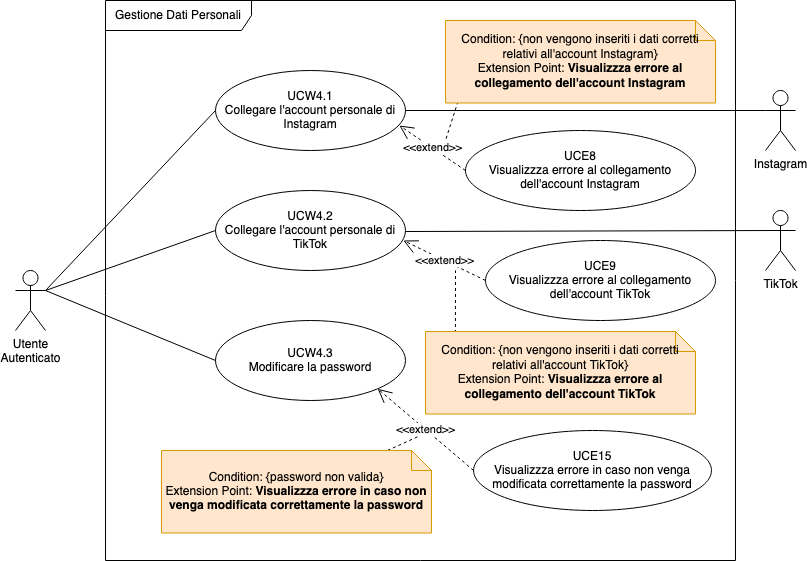
\includegraphics[scale=0.5]{UC_images/UCW4-1.png}
\caption{Sottocasi UCW4}
\end{figure}
\subsubsection{UCW4.1 - Collegare l'Account Instagram}
\begin{itemize}
\item \textbf{Descrizione}: L'utente autenticato collega il proprio account Instagram al profilo.
\item \textbf{Attore primario}: Utente autenticato.
\item \textbf{Attore secondario}: Instagram.
\item \textbf{Precondizione}: L’utente è autenticato nel sistema.
\item \textbf{Postcondizione}: L’utente ha collegato il suo account Instagram al sistema.

\item \textbf{Scenario principale}:
\begin{enumerate}
\item L’utente collega il suo account personale di Instagram;
\item Per confermare l’azione, l’utente deve cliccare su “Salva”. 
\end{enumerate}

\item \textbf{Estensioni}:
\begin{itemize}
\item Il collegamento all’account Instagram non va a buon fine
\begin{enumerate}
	\item L’utente prova a collegare il proprio account Instagram all’account registrato nel sistema, cliccando il bottone “Instagram”;
	\item L’accesso alla piattaforma Instagram non va a buon fine, poiché non vengono inseriti i dati di accesso corretti (UCE8 §3.22).
	%\item All’utente viene offerta la possibilità di effettuare un nuovo collegamento
\end{enumerate}
\end{itemize}
\end{itemize}

\subsubsection{UCW4.2 - Collegare l'Account TikTok}
\begin{itemize}
\item \textbf{Descrizione}: L'utente autenticato collega il proprio account TikTok al profilo.
\item \textbf{Attore primario}: Utente autenticato.
\item \textbf{Attore secondario}: TikTok.
\item \textbf{Precondizione}: L’utente è autenticato nel sistema.
\item \textbf{Postcondizione}: L’utente ha collegato il suo account TikTok al sistema.

\item \textbf{Scenario principale}:
\begin{enumerate}
\item L’utente collega il suo account personale di TikTok;
\item Per confermare l’azione, l’utente deve cliccare su “Salva”. 
\end{enumerate}

\item \textbf{Estensioni}:
\begin{itemize}
\item Il collegamento all’account TikTok non va a buon fine
\begin{enumerate}
	\item L’utente prova a collegare il proprio account TikTok all’account registrato nel sistema, cliccando il bottone TikTok;
	\item L’accesso alla piattaforma TikTok non va a buon fine, poiché non vengono inseriti i dati di accesso corretti (UCE9 §3.23).
\end{enumerate}
\end{itemize}
\end{itemize}

\subsubsection{UCW4.3 - Modifica della password}
\begin{itemize}
\item \textbf{Descrizione}: L'utente autenticato modifica la password con cui accedere al sistema.
\item \textbf{Attore primario}: Utente autenticato.
\item \textbf{Precondizione}: L’utente è autenticato nel sistema.
\item \textbf{Postcondizione}: L’utente ha modificato con successo la password per l’accesso al sistema.

\item \textbf{Scenario principale}:
\begin{enumerate}
\item L’utente digita la nuova password nel campo password;
\item L’utente clicca su “Salva” per aggiornare la password con cui accedere al sistema.
\end{enumerate}

\item \textbf{Estensioni}:
\begin{itemize}
\item Viene inserita una password con meno di 8 caratteri
\begin{enumerate}
	\item L'utente inserisce una password non valida (UCE15 §3.29).
\end{enumerate}
\end{itemize}
\end{itemize}

\pagebreak